\documentclass[12pt]{article}
\usepackage{amsmath}
\usepackage{graphicx}
\usepackage{hyperref}
\usepackage{listings}
\usepackage{color}
\usepackage{pythonhighlight}

\title{Operating System Course Report - First Half of the Semester}
\author{A class}
\date{\today}

\begin{document}

\maketitle
\newpage

\tableofcontents
\newpage

\section{Introduction}
This report summarizes the topics covered during the first half of the Operating System course. It includes theoretical concepts, practical implementations, and assignments. The course focuses on the fundamentals of operating systems, including system architecture, process management, CPU scheduling, and deadlock handling.

\section{Course Overview}
\subsection{Objectives}
The main objectives of this course are:
\begin{itemize}
    \item To understand the basic components and architecture of a computer system.
    \item To learn process management, scheduling, and inter-process communication.
    \item To explore file systems, input/output management, and virtualization.
    \item To study the prevention and handling of deadlocks in operating systems.
\end{itemize}

\subsection{Course Structure}
The course is divided into two halves. This report focuses on the first half, which covers:
\begin{itemize}
    \item Basic Concepts and Components of Computer Systems
    \item System Performance and Metrics
    \item System Architecture of Computer Systems
    \item Process Description and Control
    \item Scheduling Algorithms
    \item Process Creation and Termination
    \item Introduction to Threads
    \item File Systems
    \item Input and Output Management
    \item Deadlock Introduction and Prevention
    \item User Interface Management
    \item Virtualization in Operating Systems
\end{itemize}

\section{Topics Covered}

\subsection{Basic Concepts and Components of Computer Systems}
This section explains the fundamental components that make up a computer system, including the CPU, memory, storage, and input/output devices.

\subsection{System Performance and Metrics}
This section introduces various system performance metrics used to measure the efficiency of a computer system, including throughput, response time, and utilization.

\subsection{System Architecture of Computer Systems}
Describes the architecture of modern computer systems, focusing on the interaction between hardware and the operating system.

\subsection{Process Description and Control}
Processes are a central concept in operating systems. This section covers:
\begin{itemize}
    \item Process states and state transitions
    \item Process control block (PCB)
    \item Context switching
\end{itemize}

\subsection{Scheduling Algorithms}
This section covers:
\begin{itemize}
    \item First-Come, First-Served (FCFS)
    \item Shortest Job Next (SJN)
    \item Round Robin (RR)
\end{itemize}
It explains how these algorithms are used to allocate CPU time to processes.

\subsection{Process Creation and Termination}
Details how processes are created and terminated by the operating system, including:
\begin{itemize}
    \item Process spawning
    \item Process termination conditions
\end{itemize}

\subsection{Introduction to Threads}
This section introduces the concept of threads and their relation to processes, covering:
\begin{itemize}
    \item Single-threaded vs. multi-threaded processes
    \item Benefits of multithreading
\end{itemize}

\begin{figure}[h]
    \centering
    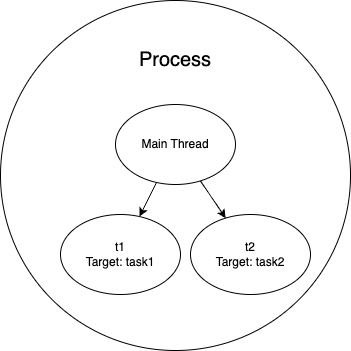
\includegraphics[width=0.5\textwidth]{/Users/khawaritzmi/Unhas/os_report_mid2024/a_class/asset/example.png}  % Sesuaikan nama file dan ukurannya
    \caption{Ini adalah gambar contoh dari multithreading.}
    \label{fig:contoh_gambar}
\end{figure}

Seperti yang terlihat pada Gambar \ref{fig:contoh_gambar}, inilah cara menambahkan gambar dengan keterangan.

\subsection{File Systems}
File systems provide a way for the operating system to store, retrieve, and manage data. This section explains:
\begin{itemize}
    \item File system structure
    \item File access methods
    \item Directory management
\end{itemize}

\subsection{Input and Output Management}
Input and output management is key for handling the interaction between the system and external devices. This section includes:
\begin{itemize}
    \item Device drivers
    \item I/O scheduling
\end{itemize}

\subsection{Deadlock Introduction and Prevention}
Explores the concept of deadlocks and methods for preventing them:
\begin{itemize}
    \item Deadlock conditions
    \item Deadlock prevention techniques
\end{itemize}

\subsection{User Interface Management}


User Interface Management adalah proses merancang, mengimplementasikan, dan memelihara elemen-elemen interaktif dari sebuah sistem perangkat lunak yang memungkinkan pengguna untuk berinteraksi dengan fungsionalitas sistem  tersebut.

\subsubsection{Jenis-Jenis User Interface}
\par antarmuka pengguna(User Interface) dapat didefinisikan sebagai bagian dari sistem komputer yang memungkinkan manusia berinteraksi dengan dan melakukan tugas-tugas pada sistem komputer tersebut. Perkembangan antarmuka pengguna telah menghasilkan beberapa jenis utama, termasuk Command Line Interface (CLI), Graphical User Interface (GUI), Text User Interface (TUI), Voice User Interface (VUI), dan Conversational User Interface (CUI). 

\begin{enumerate}
    \item{Graphical User Interface (GUI) }



\textit{Graphical User Interface} (GUI) adalah tipe antarmuka yang digunakan
oleh pengguna untuk berinteraksi dengan sistem operasi melalui gambar- gambar grafik, ikon, menu, dan menggunakan perangkat penunjuk (pointing
device) seperti mouse atau track ball. Elemen-elemen utama dari GUI bisa
diringkas dalam konsep WIMP ( window, icon, menu, pointing device)



 \item{Command Line Interface (CLI)}

\textit{Command Line Interface} (CLI) adalah tipe antarmuka dimana pengguna berinteraksi dengan sistem operasi melalui text-terminal. Pengguna menjalankan perintah dan program di sistem operasi tersebut dengan cara mengetikkan baris-baris tertentu.




\item{ Text User Interface (TUI)}

\textit{Text User Interface} (TUI) merupakan bentuk antarmuka yang menggabungkan elemen CLI dan GUI. Antarmuka ini menggunakan karakter teks untuk menciptakan tampilan semi-grafis. TUI menawarkan navigasi yang lebih mudah dibandingkan CLI, namun tetap mempertahankan efisiensi penggunaan sumber daya sistem yang rendah. TUI sering digunakan pada sistem operasi berbasis teks atau aplikasi yang memerlukan tampilan sederhana namun fungsional.

\item {Voice User Interface (VUI)}

\textit{Voice User Interface} (VUI) adalah jenis antarmuka yang memungkinkan pengguna berinteraksi dengan sistem menggunakan suara. Teknologi ini memanfaatkan pemrosesan bahasa alami dan pengenalan suara untuk menerjemahkan perintah verbal menjadi tindakan yang dapat dieksekusi oleh sistem. VUI telah menjadi semakin populer dengan munculnya asisten virtual seperti Siri, Alexa, dan Google Assistant.


\item{Conversitional User Interface (CUI)}

\textit{Conversitional User Interface} (CUI) merupakan pengembangan lebih lanjut dari VUI, yang memungkinkan interaksi yang lebih alami dan kontekstual antara pengguna dan sistem. CUI tidak hanya mengandalkan perintah suara, tetapi juga dapat menggunakan teks, seperti yang terlihat pada chatbot dan asisten virtual berbasis teks. CUI dirancang untuk memahami konteks percakapan dan memberikan respons yang lebih personal dan relevan

\end{enumerate}



\subsubsection{Interaksi antara Pengguna dan Sistem Operasi}

 Interaksi antara pengguna dan sistem operasi adalah proses komunikasi dua arah yang memungkinkan pengguna untuk mengendalikan dan menggunakan fungsi-fungsi komputer melalui berbagai jenis antarmuka. Aspek-aspek kunci dalam interaksi pengguna-sistem operasi:

\begin{enumerate}
\item Antarmuka Pengguna
     Grafis (GUI) menjadi pilihan utama bagi kebanyakan pengguna karena kemudahannya. Melalui GUI, pengguna dapat mengelola file, folder, dan aplikasi dengan mudah menggunakan mouse atau layar sentuh. Ikon, jendela, dan menu yang disediakan memungkinkan navigasi yang intuitif dalam sistem file dan pengoperasian berbagai fungsi komputer. Di sisi lain, Antarmuka Baris Perintah (CLI) tetap menjadi pilihan bagi pengguna tingkat lanjut dan administrator sistem. CLI menawarkan kontrol yang lebih presisi dan kemampuan untuk mengotomatisasi tugas-tugas kompleks melalui skrip.

\item {Manajemen File dan Direktori}
    menjadi lebih mudah dengan adanya representasi visual dalam GUI, sementara CLI menyediakan perintah-perintah yang memungkinkan manipulasi file secara efisien. Pengguna dapat dengan mudah membuat, menghapus, memindahkan, dan mengorganisir file serta folder sesuai kebutuhan mereka.

\item {Manajemen Proses}
    sistem operasi memungkinkan pengguna untuk memulai, menghentikan, dan memantau aplikasi yang berjalan. GUI menyediakan task manager yang memvisualisasikan proses yang sedang berjalan, sementara CLI menawarkan perintah-perintah untuk mengelola proses dengan tingkat kontrol yang lebih tinggi.

  \item {Konfigurasi Sistem}
     menjadi lebih accessible melalui panel kontrol atau pengaturan dalam GUI, memungkinkan pengguna untuk menyesuaikan berbagai aspek sistem operasi. Sementara itu, CLI dan Text User Interface (TUI) memungkinkan konfigurasi yang lebih mendalam melalui file konfigurasi dan perintah-perintah khusus.

  \item {Keamanan dan otentikasi}
    merupakan aspek krusial dalam interaksi pengguna-sistem. Sistem operasi menyediakan mekanisme login dan manajemen hak akses untuk melindungi data dan sumber daya sistem. GUI menawarkan dialog visual yang user-friendly untuk proses otentikasi, sementara CLI menggunakan prompt teks yang sederhana namun aman.

  \item {Pembaruan dan pemeliharaan sistem }  
    menjadi lebih mudah dengan adanya notifikasi visual dan wizard dalam GUI. Sementara itu, CLI memungkinkan administrator sistem untuk melakukan pembaruan dan pemeliharaan melalui perintah dan skrip yang dapat diotomatisasi.


 \item{Aksesibilitas} 
    menjadi fokus penting dalam pengembangan antarmuka modern. Voice User Interface (VUI) dan Conversational User Interface (CUI) meningkatkan aksesibilitas bagi pengguna dengan kebutuhan khusus. Fitur seperti pembaca layar dan kontrol suara terintegrasi dengan baik dalam sistem operasi modern, memastikan bahwa teknologi dapat diakses oleh semua kalangan.
\end{enumerate}

\begin{thebibliography}{9} 

\bibitem{Shneiderman2016}
Shneiderman, B., Plaisant, C., Cohen, M., Jacobs, S., Elmqvist, N., \& Diakopoulos, N. (2016). \textit{Designing the User Interface: Strategies for Effective Human-Computer Interaction} (6th ed.). Pearson.

\bibitem{McTear2016}
McTear, M., Callejas, Z., \& Griol, D. (2016). \textit{The conversational interface: Talking to smart devices}. Springer.

\bibitem{Raymond2003}
Raymond, E. S. (2003). \textit{The art of Unix programming}. Addison--Wesley Professional. 

\bibitem{Cohen2004}
Cohen, M. H., Giangola, J. P., \& Balogh, J. (2004). \textit{Voice user interface design}. Addison--Wesley Professional.

\bibitem{Reynaldi2019}
Reynaldi, A. (2019). \textit{Perancangan desain antarmuka pengguna (UI) aplikasi pencari kos} [Skripsi tidak diterbitkan]. Program Studi Desain Komunikasi Visual, Fakultas Seni dan Desain, Universitas Negeri Makassar


			

\end{thebibliography}




\subsection{Virtualization in Operating Systems}
Virtualization allows multiple operating systems to run concurrently on a single physical machine. This section explores:
\begin{itemize}
    \item Concept of virtualization
    \item Hypervisors and their types
    \item Benefits of virtualization in modern computing
\end{itemize}

\section{Assignments and Practical Work}
\subsection{Assignment 1: Process Scheduling}
Students were tasked with implementing various process scheduling algorithms (e.g., FCFS, SJN, and RR) and comparing their performance under different conditions.
\subsubsection{Group 1}
\begin{python}
    class Process:
    def __init__(self, pid, arrival_time, burst_time):
        self.pid = pid
        self.arrival_time = arrival_time
        self.burst_time = burst_time
        self.completion_time = 0
        self.turnaround_time = 0
        self.waiting_time = 0
\end{python}

\subsubsection{Kelompok 12}

\paragraph{Pertanyaan:}Diberikan tiga proses dengan waktu kedatangan dan waktu eksekusi sebagai berikut:

\begin{itemize}
    \item Proses A:
    \begin{itemize}
        \item Kedatangan: 0 ms
        \item Eksekusi: 8 ms
    \end{itemize}
    \item Proses B:
    \begin{itemize}
        \item Kedatangan: 1 ms
        \item Eksekusi: 4 ms
    \end{itemize}
    \item Proses C:
    \begin{itemize}
        \item Kedatangan: 2 ms
        \item Eksekusi: 9 ms
    \end{itemize}
\end{itemize}

\subsubsection{Perhitungan Waktu Penyelesaian}

\begin{itemize}
    \item Proses A:
    \begin{itemize}
        \item Kedatangan: 0 ms
        \item Eksekusi: 8 ms
        \item Waktu Penyelesaian: 0 ms + 8 ms = 8 ms
    \end{itemize}
    \item Proses B:
    \begin{itemize}
        \item Kedatangan: 1 ms
        \item Eksekusi: 4 ms
        \item Waktu Penyelesaian: 8 ms (waktu penyelesaian Proses A) + 4 ms = 12 ms
    \end{itemize}
    \item Proses C:
    \begin{itemize}
        \item Kedatangan: 2 ms
        \item Eksekusi: 9 ms
        \item Waktu Penyelesaian: 12 ms (waktu penyelesaian Proses B) + 9 ms = 21 ms
    \end{itemize}
\end{itemize}

\subsubsection{Tabel Waktu Penyelesaian}

\begin{table}[h]
\centering
\begin{tabular}{|c|c|}
\hline
\textbf{Proses} & \textbf{Waktu Penyelesaian (Completion Time)} \\
\hline
A & 8 ms \\
\hline
B & 12 ms \\
\hline
C & 21 ms \\
\hline
\end{tabular}
\caption{Waktu Penyelesaian Proses}
\label{tab:completion_time}
\end{table}

\begin{table}[htbp] % Optional: For floating position
    \centering
    \begin{tabular}{|c|c|c|} % Defines number of columns and alignment (c = center, l = left, r = right). '|' creates vertical lines.
    \hline
    Header 1 & Header 2 & Header 3 \\ % Column headers
    \hline
    Row 1, Column 1 & Row 1, Column 2 & Row 1, Column 3 \\ % First row of data
    \hline
    Row 2, Column 1 & Row 2, Column 2 & Row 2, Column 3 \\ % Second row of data
    \hline
    \end{tabular}
    \caption{Your table caption} % Optional: For adding a caption
    \label{tab:your_label} % Optional: For cross-referencing the table
\end{table}
\subsection{Assignment 2: Deadlock Handling}
In this assignment, students were asked to simulate different deadlock scenarios and explore various prevention methods.


\subsubsection{Group 12}

\paragraph{Pertanyaan:} Jelaskan perbedaan antara metode pencegahan dan metode penanganan deadlock!

\paragraph{Jawaban:} 
\begin{itemize}
    \item Pencegahan Deadlock: Metode ini berusaha mencegah deadlock dengan memastikan bahwa setidaknya satu dari empat kondisi deadlock tidak pernah terjadi. Misalnya, dengan menggunakan alokasi sumber daya secara hati-hati sehingga tidak ada proses yang dapat menahan dan menunggu sumber daya lainnya (melanggar kondisi "hold and wait").

    \item Penanganan Deadlock: Metode ini membiarkan deadlock terjadi, kemudian mendeteksinya, dan mengambil langkah-langkah untuk menyelesaikan situasi tersebut. Misalnya, dengan membatalkan salah satu atau beberapa proses untuk memutus siklus deadlock.
\end{itemize}



\subsection{Assignment 3: Multithreading and Amdahl's Law}
This assignment involved designing a multithreading scenario to solve a computationally intensive problem. Students then applied **Amdahl's Law** to calculate the theoretical speedup of the program as the number of threads increased.
\subsubsection{Kelompok 12}
\paragraph{Pertanyaan:} Mengapa speedup dari program paralel tidak terus meningkat secara linear seiring dengan peningkatan jumlah thread? Jelaskan berdasarkan Amdahl's Law.

\paragraph{Jawaban:} Berdasarkan Amdahl's Law, peningkatan jumlah thread tidak menghasilkan peningkatan speedup secara linear karena selalu ada bagian dari program yang tidak dapat diparalelkan (bagian serial). Meskipun jumlah thread ditingkatkan, bagian serial tersebut tetap menjadi penghambat sehingga membatasi peningkatan speedup secara keseluruhan. Saat jumlah thread meningkat, kontribusi bagian serial semakin dominan, sehingga limitasi ini menyebabkan speedup mendekati nilai maksimum tertentu, tetapi tidak terus meningkat secara linear.

Berdasarkan Amdahl's Law, peningkatan jumlah thread tidak menghasilkan peningkatan speedup secara linear karena selalu ada bagian dari program yang tidak dapat diparalelkan (bagian serial). Meskipun jumlah thread ditingkatkan, bagian serial tersebut tetap menjadi penghambat sehingga membatasi peningkatan speedup secara keseluruhan. Saat jumlah thread meningkat, kontribusi bagian serial semakin dominan, sehingga limitasi ini menyebabkan speedup mendekati nilai maksimum tertentu, tetapi tidak terus meningkat secara linear.


\subsection{Assignment 4: Simple Command-Line Interface (CLI) for User Interface Management}
Students were tasked with creating a simple **CLI** for user interface management. The CLI should support basic commands such as file manipulation (creating, listing, and deleting files), process management, and system status reporting.

\subsubsection{Kelompok 12}

\paragraph{Pertanyaan:} Mahasiswa diminta untuk membuat antarmuka baris perintah sederhana (CLI) yang dapat digunakan untuk mengelola antarmuka pengguna. CLI ini harus mendukung perintah dasar seperti manipulasi file (membuat, menampilkan, dan menghapus file), manajemen proses, dan pelaporan status sistem.

\paragraph{Jawab:} Berikut adalah implementasi CLI dalam Python:

\begin{lstlisting}[language=Python]
import os
import psutil

def create_file(filename):
    with open(filename, 'w') as f:
        f.write('')  # Create an empty file
    print(f'File {filename} created successfully.')

def list_files():
    files = os.listdir()
    if files:
        print("Files in the current directory:")
        for file in files:
            print(f' - {file}')
    else:
        print("No files found in the current directory.")

def delete_file(filename):
    try:
        os.remove(filename)
        print(f'File {filename} deleted successfully.')
    except FileNotFoundError:
        print(f'File {filename} not found.')
    except Exception as e:
        print(f'Error deleting file: {e}')

def show_processes():
    print("Currently running processes:")
    for proc in psutil.process_iter(['pid', 'name']):
        print(f' - PID: {proc.info["pid"]}, Name: {proc.info["name"]}')

def show_system_status():
    print("System Status:")
    print(f' - Total Memory: {psutil.virtual_memory().total // (1024 ** 2)} MB')
    print(f' - Available Memory: {psutil.virtual_memory().available // (1024 ** 2)} MB')
    print(f' - Used Memory: {psutil.virtual_memory().used // (1024 ** 2)} MB')
    print(f' - CPU Usage: {psutil.cpu_percent(interval=1)}%')

def main():
    while True:
        command = input("Enter command (create, list, delete, processes, status, exit): ").strip().lower()
        if command.startswith("create "):
            filename = command.split(" ", 1)[1]
            create_file(filename)
        elif command == "list":
            list_files()
        elif command.startswith("delete "):
            filename = command.split(" ", 1)[1]
            delete_file(filename)
        elif command == "processes":
            show_processes()
        elif command == "status":
            show_system_status()
        elif command == "exit":
            print("Exiting the CLI.")
            break
        else:
            print("Invalid command. Please try again.")

if __name__ == "__main__":
    main()
\end{lstlisting}

\paragraph{Penjelasan:} Program ini mengimplementasikan CLI sederhana dengan fungsi-fungsi berikut:
\begin{itemize}
    \item \texttt{create\_file}: Membuat file kosong dengan nama yang ditentukan.
    \item \texttt{list\_files}: Menampilkan daftar file dalam direktori saat ini.
    \item \texttt{delete\_file}: Menghapus file dengan nama yang ditentukan.
    \item \texttt{show\_processes}: Menampilkan daftar proses yang sedang berjalan.
    \item \texttt{show\_system\_status}: Menampilkan status sistem, termasuk penggunaan memori dan CPU.
\end{itemize}

Program utama (\texttt{main}) menjalankan loop yang terus meminta input perintah dari pengguna dan menjalankan fungsi yang sesuai berdasarkan perintah tersebut.





\subsection{Assignment 5: File System Access}
In this assignment, students implemented file system access routines, including:
\begin{itemize}
    \item File creation and deletion
    \item Reading from and writing to files
    \item Navigating directories and managing file permissions
\end{itemize}

\subsubsection{Kelompok 12}b

\paragraph{Pertanyaan:} Bagaimana mekanisme pengaturan izin akses langsung ke sistem berkas lokal dari aplikasi web melalui API File System Access dalam konteks keamanan data, dan bagaimana cara pengembang dapat memastikan bahwa izin yang diberikan kepada aplikasi hanya terbatas pada direktori yang spesifik tanpa menimbulkan potensi risiko pengungkapan data di luar cakupan yang dimaksud?

\paragraph{Jawaban:} Mekanisme pengaturan izin akses dalam File System Access API memungkinkan aplikasi web untuk berinteraksi langsung dengan sistem berkas lokal pengguna. Akses ini dilakukan berdasarkan izin yang diberikan pengguna secara eksplisit, sehingga pengembang harus memastikan aplikasi hanya meminta izin untuk berkas atau direktori yang diperlukan.

Untuk meningkatkan keamanan, penting untuk menerapkan scoped access permissions agar aplikasi tidak dapat mengakses berkas di luar cakupan izin. Pengembang juga perlu waspada terhadap potensi serangan seperti directory traversal attacks dengan melakukan path sanitization. Penggunaan persisted permissions harus dikelola dengan hati-hati agar tidak mengorbankan privasi pengguna. Dengan langkah-langkah ini, aplikasi dapat berfungsi efektif tanpa risiko mengungkapkan data sensitif.



\section{Conclusion}
The first half of the course introduced core operating system concepts, including process management, scheduling, multithreading, and file system access. These topics provided a foundation for more advanced topics to be covered in the second half of the course.

\end{document}